\section{Durchführung}
\label{sec:Durchführung}

Der Versuchaufbau ist in Abbildung \ref{fig:aufbau} zu sehen. Dabei ist die  genaue Justierung
der dargestellten Elemente von großer Bedeutung, da nur sehr geringe Ströme gemessen
werden.

\begin{figure}
  \centering
  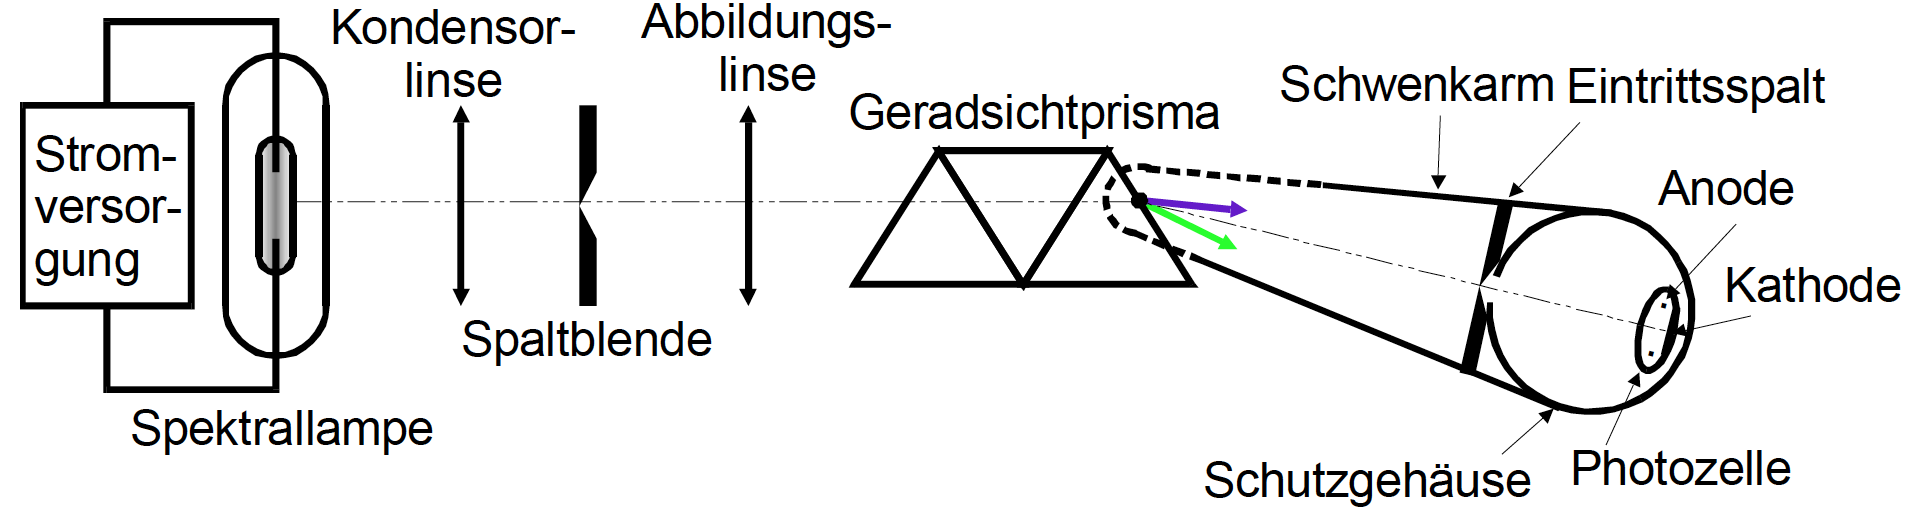
\includegraphics[width=\textwidth]{data/aufbau.png}
  \caption{Skizze des Versuchsaufbaus \cite{Versuchsanleitung}.}
  \label{fig:aufbau}
\end{figure}

Die Photozelle wird nacheinander mit monochromatischem Licht verschiedener Wellenlängen
bestrahlt und es wird jeweils der Phototstrom in Abhängigkeit von der angelegten
Gegenspannung gemessen.

Außerdem wird für Licht der Wellenlänge $\lambda=578\,$nm der Photostrom für Spannungen
in einem Bereich von $U=-19\,$V bis $U=19\,$V gemessen \footnote{Ursprünglich sollte das Intervall
gerade bei $\SI{-20}{\volt}$ beginnen und bei $\SI{20}{\volt}$ enden. Da dies jedoch mit
dem Gerät nicht möglich war, wurde das angegebene Intervall gewählt.}.
